\section{Лекция 18 (30.11)}

\subsection{Нестационарное уравнение Навье-Стокса}
\label{sec:ns2d-nonstat}

Запишем безразмерную систему \eqref{eq:ns2d_u} -- \eqref{eq:ns2d_div} в нестационарной постановке
\begin{equation}
\label{eq:ns2d_nonstat}
\begin{array}{l}
    \ddfr{u}{t} + \ddfr{u^2}{x} + \ddfr{uv}{y} =
        -\ddfr{p}{x}
        + \dfrac{1}{\Ren}\left(\ddfrq{u}{x} + \ddfrq{u}{y}\right),\\[10pt]
    \ddfr{v}{t} + \ddfr{uv}{x} + \ddfr{v^2}{y} =
        -\ddfr{p}{y}
        + \dfrac{1}{\Ren}\left(\ddfrq{v}{x} + \ddfrq{v}{y}\right), \\[10pt]
    \ddfr{u}{x} + \ddfr{v}{y} = 0.
\end{array}
\end{equation}
Характерное время, на которое было произведено обезразмериваение,
равно $t^0 = L/U$.

\subsubsection{Cхема расчёта по алгоритму SIMPLE}
\label{sec:simple-nonstat-algo}

Производную по времени будет аппроксимировать по двухслойной неявной схеме.
\begin{equation*}
\dfr{u}{t} = \frac{\hat u - \check u}{\dt} + o(\dt),
\end{equation*}
где символом $\check\cdot$ обозначены значения с предыдущего временн\'{о}го слоя.

Внутри каждого временн\'{о}го слоя будем исполнять
итерационный процесс по типу \eqref{eq:ns2d_semi_u} -- \eqref{eq:ns2d_semi_div}
с добавлением дискретизованной производной по времени:

\begin{equation}
    \label{eq:ns2d_nonstat_semi}
    \begin{array}{l}
    \displaystyle
    \frac{\hat u - \check u}{\dt} + \frac{\hat u - u}{\tau} + \dfr{u \hat u}{x} + \dfr{v \hat u}{y} =
        -\dfr{\hat p}{x}
        + \frac{1}{\Ren}\left(\dfrq{\hat u}{x} + \dfrq{\hat u}{y}\right), \\[10pt]
    \displaystyle
    \frac{\hat v - \check v}{\dt} + \frac{\hat v - v}{\tau} + \dfr{u\hat v}{x} + \dfr{v \hat v}{y} =
        -\dfr{\hat p}{y}
        + \frac{1}{\Ren}\left(\dfrq{\hat v}{x} + \dfrq{\hat v}{y}\right),  \\[10pt]
    \displaystyle
    \dfr{\hat u}{x} + \dfr{\hat v}{y} = 0.
    \end{array}
\end{equation}

Далее на основе этих уравнений проведём рассуждения, аналогичные приведённым в п. \ref{sec:simple-algo}.
Уравнения для пробной скорости типа \eqref{eq:ns2d_ustar}, \eqref{eq:ns2d_vstar}
примут вид
\begin{equation}
    \label{eq:ns2d_nonstat_uvstar}
    \begin{array}{l}
    \displaystyle
    \left(1 + \frac{\tau}{\dt}\right)u^* + \tau\dfr{u u^*}{x} + \tau\dfr{v u^*}{y}
       - \frac{\tau}{\Ren}\left(\dfrq{u^*}{x} + \dfrq{u^*}{y}\right)
       = -\tau\dfr{p}{x} + u + \frac\tau\dt \check u, \\[10pt]
    \displaystyle
    \left(1 + \frac{\tau}{\dt}\right)v^* + \tau\dfr{u v^*}{x} + \tau\dfr{v v^*}{y}
       - \frac{\tau}{\Ren}\left(\dfrq{v^*}{x} + \dfrq{v^*}{y}\right)
       = -\tau\dfr{p}{y} + v + \frac\tau\dt \check v.
   \end{array}
\end{equation}

Уравнения для поправок скорости \eqref{eq:ns2d_uprime_approx}, \eqref{eq:ns2d_vprime_approx}
и давления \eqref{eq:ns2d_pprime_diff}
можно оставить в неизменном виде если модифицировать входящие в них множители $d^u, d^v$.
По аналогии с \eqref{eq:ns2d_du}, \eqref{eq:ns2d_dv} запишем
\begin{equation}
    \label{eq:ns2d_nonstat_duv}
    \begin{array}{l}
    \displaystyle
    d^u = \left({\rm diag}\left(S^u\right)\right)^{-1} = 
        \left(1 + \frac\tau\dt + \frac{2\tau}{\Ren}\left(\frac{1}{h_x^2} + \frac{1}{h_y^2}\right)\right)^{-1} \\[10pt]
    \displaystyle
    d^v = \left({\rm diag}\left(S^v\right) \right)^{-1}= 
        \left(1 + \frac\tau\dt + \frac{2\tau}{\Ren}\left(\frac{1}{h_x^2} + \frac{1}{h_y^2}\right)\right)^{-1}.
    \end{array}
\end{equation}
Здесь $S^u$, $S^v$ -- матрицы левых частей выражений \eqref{eq:ns2d_nonstat_uvstar}.

Схема расчёта на временн\'{о}м слое остаётся аналогичной стационарному случаю,
с той разницей, что первая итерация использует значение расчётных полей
с предыдущего шага по времени.
Порядок действий на временном слое:

\begin{enumerate}
\item Присвоить $u=\check u$, $v=\check v$, $p=\check p$;
\item Из уравнений \eqref{eq:ns2d_nonstat_uvstar}
      вычислить значения $u^*, v^*$;
\item Определить поправку давления $p'$ из уравнения \eqref{eq:ns2d_pprime_diff} с использованием \eqref{eq:ns2d_nonstat_duv};
\item Найти поправки скорости $u', v'$ из выражений \eqref{eq:ns2d_uprime_approx}, \eqref{eq:ns2d_vprime_approx} с использованием \eqref{eq:ns2d_nonstat_duv};
\item Выразить значения переменных для текущего слоя из \eqref{eq:ns2d_decomp};
      Для определения давления использовать сглаживание с коэффициентом $\alpha_p$;
\item Найти невязку с ипользованием найденных значений $\hat u, \hat v, \hat p$
      из выражения \eqref{eq:ns2d_residual}.
      Если она недостаточно мала, то выполняется присваивание
      $u = \hat u, \; v=\hat v, \; p = \hat p$ 
      и возвращение на шаг 2.
      Если сходимость достигнута, то перейти на следующий шаг по времени.
      Для этого выполнить
      $\check u = \hat u, \; \check v= \hat v, \; \check p = \hat p$ 
      и перейти на шаг 1.
\end{enumerate}

\subsection{Задача об обтекании препятствия}
\label{sec:problem-obstacle}

\subsubsection{Расчётная сетка}
Рассмотрим постановку граничных условий и особенности пространственной аппроксимации для задачи
о внешнем обтекании. Поскольку рассматриваемые нами методы
пока ограничены аппроксимациями на структурированной прямоугольной
сетке, то будем рассматривать такую область расчёта,
которую легко можно отобразить на такой сетке. Пусть внешняя
область расчёта и обтекаемое препятствие представляет из себя прямоугольники.

\begin{figure}[h!]
\centering
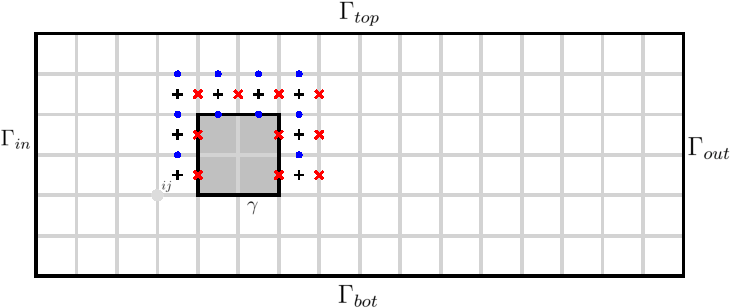
\includegraphics[width=0.8\linewidth]{obstacle_staggered.pdf}
\caption{Область расчёта и разнесённая сетка для задачи обтекания}
\label{fig:obstacle_staggered}
\end{figure}

По аналогии с \figref{fig:staggered_grid} введём в этой области
прямоугольную сетку (\figref{fig:obstacle_staggered}).

В случае сохранения естестественной нумерации узлов и ячеек сетки
часть их этих пронумерованных ячеек выпадает из области расчёта (попадает внутрь препятствия).
Для таких случаев существует два способа работы с нумерацией:
\begin{itemize}
\item
Можно сохранить естественную нумерацию, при этом часть ячеек пометить
как неактивные (например, введя специальный массив признаков \ename{actnum},
$i$-ый элемент которого равен единице для активной ячейки и нулю для неактивной).
Количество элементов в сеточных векторах тогда будет равно общему количеству
всех ячеек (и активных и неактивных). Но значения этих векторов в неактивных ячейках будут фиктивными (нулями).
\item
Можно нумеровать лишь активные ячейки (и узлы), тем самым
нарушив естественную нумерацию. 
\end{itemize}

Оба этих подхода имеют свои очевидные плюсы и минусы.
Первый подход сохраняет простые зависимости для перевода двумерного индекса в сквозной и
диагональную структуру сеточных матриц. Второй подход более экономичен в хранении данных. 

\subsubsection{Граничные условия}
Рассмотрим постановку со следующими граничными условиями:
\begin{itemize}
\item
во входном сечении зададим равномерный профиль скорости
\begin{equation}
\label{eq:ns2d_obstable_bc_in}
(x, y) \in \Gamma_{in}: u=1, \; v=0;
\end{equation}
\item
на нижней и верхней границах -- условие симметрии (идеального скольжения). Это условие моделирует
зеркальное отражение расчётной области относительно соответствующих границ $\Gamma_{top}, \Gamma_{bot}$.
\begin{equation}
\label{eq:ns2d_obstable_bc_topbot}
(x, y) \in \Gamma_{top}, \Gamma_{bot}: \dfr{u}{n}=0, \; v = 0;
\end{equation}
\item
на самом обтекаемом деле -- условия прилипания
\begin{equation}
\label{eq:ns2d_obstable_bc_wall}
(x,y) \in \gamma: u=0, \; v=0;
\end{equation}
\item
в выходном сечении -- условия выхода потока. Их точную формулировку определим позднее.
\end{itemize}

На каждом шаге алогоритма SIMPLE требуется
решить три дифференциальных уравнения \cref{eq:ns2d_ustar,eq:ns2d_vstar,eq:ns2d_pprime_diff}.
относительно неизвестных $u^*, v^*, p'$.
Значит из представленных выше граничных условий требуется
выразить граничные значения для этих трёх неизвестных сеточных векторов
и расписать способ их учёта при сборке соответствующих систем линейных уравнений.

\subsubsubsection{Входное сечение}
\label{sec:obstacle_bc_input}
При разложении скорости на пробное значение и поправку \cref{eq:ns2d_decomp}
условия для скорости \cref{eq:ns2d_obstable_bc_in} раскладываются следующим образом:
\begin{equation}
\label{eq:ns2d_decomp_input}
(x,y) \in \Gamma_{in}: u^* = 1, \; v^* = 0, \; u' = v' = 0
\end{equation}
Условия первого рода для пробной скорости учитываются при решении уравнений
\cref{eq:ns2d_ustar,eq:ns2d_vstar}.
Для сеточного вектора $u^*$, узлы которого лежат непосредственно на границе,
учёт этого условия сводится к модификации соответствующей строки матрицы $A^u$ и правой части $b^u$.
В строке $k=k\left[0, j+\tfrac12\right]$:
\begin{equation}
\label{eq:ns2d_au_bc_left}
A^u_{km} = \delta_{km}, \quad b^u_k = 1.
\end{equation}

Для сеточного вектора $v^*$ учёт производится с помощью выражения для значения в фиктивном узле $k_1 = k\left[-\tfrac12, j\right]$
через значение в настоящем узле $k_0 = k\left[\tfrac12, j\right]$:
$$
\frac{v^*_{k_0} + v^*_{k_1}}{2} = 0 \hence v^*_{k_1} = -v^*_{k_0}.
$$
Поэтому при сборке матрицы $A^v$ по формулам \cref{eq:ns2d_av} при необходимости добавить
значение $a$ в колонку, соответствующую фиктивному узлу, требуется добавить это значение
в диагональ с обратным знаком:
\begin{equation}
\label{eq:ns2d_av_bc_left}
A^v_{k_0, k_1} {{+}{=}} a \hence A^v_{k_0, k_0} \minuseq a
\end{equation}

Из условий на поправку скорости $u'=v'=0$ и уравнений \cref{eq:ns2d_uprime_approx,eq:ns2d_vprime_approx}
следует граничное условие для поправки давления
\begin{equation}
\label{eq:ns2d_obstacle_bc_pres}
x,y\in\Gamma_{in}: \dfr{p'}{x}=0
\end{equation}
Из этого условия получаем соотношение для давления в фиктивном узле $k_1 = k\left[-\tfrac12, j+\tfrac12\right]$
через значение  в реальном узле $k_0 = k\left[\tfrac12, j+\tfrac12\right]$:
$$
p'_{k_1} = p'_{k_0}
$$
Тогда добавление значения $a$ в фиктивную колонку $k_1$ эквивалентно
\begin{equation}
\label{eq:ns2d_ap_bc}
A^p_{k_0, k_1} {{+}{=}} a \hence A^p_{k_0, k_0} \pluseq a
\end{equation}

Следует понимать, что выражение \cref{eq:ns2d_uprime_approx}
является приближением, используемым в расчётной схеме SIMPLE.
В действительности, использование условия \cref{eq:ns2d_obstacle_bc_pres} (в случае нулевого начального приближения давления)
приводит к нулевой производной для всего давления (а не только поправки)
$$
x,y\in\Gamma_{in}: \dfr{p}{x}=0.
$$
Это выражение никак не следует из постановки задачи.
Действительно, если расписать уравнение \cref{eq:ns2d_u} с учётом условий \cref{eq:ns2d_obstable_bc_in}
и уравнения неразрывности \cref{eq:ns2d_div}, то получим соотношение
\begin{equation}
\label{eq:ns2d_obstacle_true_bc_p}
x,y\in\Gamma_{in}: \dfr{p}{x} = \frac{1}{\Ren}\dfrq{u}{x} = -\frac1\Ren\dfr{}{x}\left(\dfr{v}{y}\right).
\end{equation}
(при выводы учтено, что $\dsfr{v}{y} = -\dsfr{u}{x} = 0$).
Однако, практика показывает, что в большинстве случаев, условий типа \cref{eq:ns2d_obstacle_bc_pres}
оказывается достаточно. Выражение \cref{eq:ns2d_obstacle_true_bc_p} равно нулю,
если поперечная компонента скорости не появляется сразу за входным сечением. То есть
течение остается прямолинейным на начальном участке расчётной области.
Чтобы это исполнялось, входное сечение необходимо размещать
на таком растоянии от препятствия, на котором поток еще не чувствует его присутствия (не начинает разворачиваться).

\subsubsubsection{Условия симметрии}
Однородные условие для скорости \cref{eq:ns2d_obstable_bc_topbot} расписываются
как
$$
(x,y) \in \Gamma_{in}: \dfr{u^*}{y} = \dfr{u'}{y} = 0, \; v^* = v' = 0.
$$
Из условия на $u^*$ запишем соотношение для фиктивного узла около нижней границы, которое будем использовать
при сборке матрицы $A^u$:
\begin{align*}
&k_0 = k\left[i+\tfrac12, \tfrac12\right], \quad k_1 = k\left[i+\tfrac12, -\tfrac12\right], \\
&u^*_{k_1} = u^*_{k_0}, \\
&A^u_{k_0, k_1} {{+}{=}} a \hence A^u_{k_0, k_0} \pluseq a.
\end{align*}
Условие на $v^*$ можно использовать явно:
\begin{align*}
&k = k\left[i+\tfrac12, \tfrac12\right], \\
&A^u_{k,s} = \delta_{ks}, \quad b^u_k = 0.
\end{align*}

Граничное условие для поправки давления
можно получить из уравнения движения \cref{eq:ns2d_v} (в неконсервативном виде) с учётом уравнения неразрывности.
Используя
\begin{align*}
&(x,y) \in \Gamma_{top,bot}:
	v = 0 \hence \dfr{v}{x} = 0 \hence \dfrq{v}{x} = 0,\\
&\phantom{(x,y) \in \Gamma_{top,bot}}:
	\dfr{u}{y} = 0 \hence \dfr{}{x}\dfr{u}{y} = 0 \hence \dfrq{v}{y} = 0,\\
\end{align*}
получим
$$
(x,y) \in \Gamma_{top,bot}: \dfr{p}{y} = 0.
$$
При использовании нулевого начального приближения давления, для поправки давления так же справедливо
$$
(x,y) \in \Gamma_{top,bot}: \dfr{p'}{y} = 0.
$$
Учёт этого условия на матричном уровне аналогичен процедуре \cref{eq:ns2d_ap_bc}.

\subsubsubsection{Условия прилипания}
\label{sec:obstacle-noslip}
Учёт условий прилипания на границе обтекаемого тела \cref{eq:ns2d_obstable_bc_wall}
в целом аналогичен алгоритму учёта входной границы.
Для компонент скорости, узлы которых лежат на границе работает процедура \cref{eq:ns2d_au_bc_left} (с нулём в правой части).
В случае если узлы не лежат на границе, то используется процедура \cref{eq:ns2d_av_bc_left}.

Для поправки давления так же используется однородное условие второго рода \cref{eq:ns2d_obstacle_bc_pres}
И все комментарии к этому условию, указанные в пункте \ref{sec:obstacle_bc_input}, остаются справедливыми.

\subsubsubsection{Выходные граничные условия}
На выходной границе отсутствует возможность указать какие-либо физичные условия для искомых переменных.
При этом, как правило, поведение течения в этой области большого интереса не представляет.
Поэтому здесь требуется написать такие выражения, учёт которых
не оказывал бы влияния на течение в основной области расчёта.
Отсюда возникает проблема формулировки неотражающих граничных условий.
Цель состоит в том, чтобы жидкость выходила из области расчёта естественным для себя образом, не подстраиваясь под выходную границу.

Простейшим решением этой проблемы является использование уравнения переноса на выходной границе:
\begin{equation}
\label{eq:ns2d_outflow_common}
\begin{aligned}
(x,y)\in\Gamma_{out}:\; &\dfr{u}{t} + u\dfr{u}{x} = 0,\\[10pt]
                        &\dfr{v}{t} + u\dfr{v}{x} = 0.
\end{aligned}
\end{equation}
В стационарном случае ($\dsfr{u,v}{t} = 0$) из этих условий следует, что поперечная скорость равна нулю:
\begin{equation*}
\dfr{u}{x} = 0 \hence \dfr{v}{y} = 0 \hence v = v|_{\Gamma_{bot}} = 0.
\end{equation*}

По аналогии с уравнениями движения \cref{eq:ns2d_semi_u}
в уравнение на выходной границе так же добавим фиктивную производную по времени.
Тогда условия для компонент скорости на итерации SIMPLE примут вид (для стационарного случая)

\begin{equation}
\label{eq:ns2d_outflow_common_semi}
\begin{aligned}
(x,y)\in\Gamma_{out}:\; &\frac{\hat u - u}{\tau} + u\dfr{\hat u}{x} = 0,\\[10pt]
                        &\hat v = 0.
\end{aligned}
\end{equation}

Подставим разложение \cref{eq:ns2d_decomp} и запишем условия для уравнений пробной скорости

\begin{align}
\label{eq:ns2d_outflow_ustar}
(x,y)\in\Gamma_{out}:\; &u^* + \tau u\dfr{u^*}{x} = u,\\[10pt]
\label{eq:ns2d_outflow_vstar}
                        &v^* = 0.
\end{align}

Пробная скорость в алгоритме SIMPLE не удовлетворяет уравнению неразрывности.
Поэтому нет гарантий, что найденная $u^*$ сохраняет баланс масса в расчётной области.
На практике это означает, что количество жидкости, которое втекает через $\Gamma_{in}$ не равно
количеству жидкости, которое вытекает через $\Gamma_{out}$.

Но финальная по итогам SIMPLE итерации скорость должна сохранять баланс массы.
То есть
$$
\triangle Q = \int_{\Gamma_{in}} \hat u \, ds - \int_{\Gamma_{out}} \hat u \, ds = 0.
$$
Раскладывая это выражение через пробную скорость и поправку с учётом нулевого значения $u'$ на входной границе \cref{eq:ns2d_decomp_input},
получим
$$
\int_{\Gamma_{out}} u' \, ds = \int_{\Gamma_{in}} u^* \, ds - \int_{\Gamma_{out}} u^* \, ds
$$
Положим, что $u'$ на выходной границе постоянна.
Это предположение не влияет на итоговый результат SIMPLE итераций, так как
при его сходимости поправки скорости обнуляются. Тогда запишем значение поправки скорости
на выходной границе
\begin{equation}
\label{eq:ns2d_uprime_from_balance}
(x,y)\in\Gamma_{out}:\; u' = \left(\int_{\Gamma_{in}} u^* \, ds - \int_{\Gamma_{out}} u^* \, ds \right) / \left|\Gamma_{out}\right|
\end{equation}
Подставляя это выражение в \cref{eq:ns2d_uprime_approx}, получим граничные условия на поправку давления
\begin{equation}
\label{eq:ns2d_outflow_pprime}
(x,y)\in\Gamma_{out}:\;  d^u\dfr{p'}{x} = -\frac{u'}{\tau}
\end{equation}

Таким образом, мы вывели граничные условия для всех трёх дифференциальных уравнений:
\cref{eq:ns2d_outflow_ustar,eq:ns2d_outflow_vstar,eq:ns2d_outflow_pprime}.

Отметим, что если выходных границ несколько, то выражение \cref{eq:ns2d_uprime_from_balance}
следует записывать для каждой из границ. При этом следует дополнительно задавать
долю расхода $C_i$, вытекающую через каждую из границ. Пусть $\Gamma_{out} = \Gamma_{o1} \cap \Gamma_{o2}$.
Тогда
\begin{align*}
&(x,y)\in\Gamma_{o1}:\; u' = \left(C_1 \int_{\Gamma_{in}} u^* \, ds - \int_{\Gamma_{o2}} u^* \, ds \right) / \left|\Gamma_{o1}\right|\\
&(x,y)\in\Gamma_{o2}:\; u' = \left(C_2 \int_{\Gamma_{in}} u^* \, ds - \int_{\Gamma_{o1}} u^* \, ds \right) / \left|\Gamma_{o2}\right|\\
&C_1 + C_2 = 1.
\end{align*}

\paragraph{Учёт условия для $u^*$ \cref{eq:ns2d_outflow_ustar}}
Просто перепишем уравнение в строках СЛАУ, соответствующих выходным узлам $k_0 = k\left[n_x, j+\tfrac12\right]$.
Для этого аппроксимируем конвективную производную по схеме против потока (с противопоточным узлом
$k_1 = k\left[n_x-1, j+\tfrac12\right]$).
$$
u^*_{k_0} + \tau U_{k_0} \frac{u^*_{k_0} - u^*_{k_1}}{h_x} = u_{k_0},
$$
где $U$ - скорость переноса в $k_0$-ом узле. Она должна быть всегда больше нуля (иначе схема
перестаёт быть противопотоковой). Можно просто положить её равной среднерасходной (единице в нашем случае).
А можно взять из предыдущей итерации с проверкой на положительность:
$$
U_{k_0} = \max\left(0, u_{k_0}\right).
$$
На матричном уровне получим:
\begin{equation}
\label{eq:ns2d_outflow_ustar_mat}
\begin{aligned}
&A^u_{k0, s} = \begin{cases}
	1 + \dfrac{\tau U_{k_0}}{h_x}, \quad s = k_0\\[10pt]
	-\dfrac{\tau U_{k_0}}{h_x}, \quad s = k_1\\[10pt]
	0, \quad \text{иначе},
\end{cases}, \\
&b^u_{k_0} = u_{k_0}
\end{aligned}
\end{equation}

\paragraph{Учёт условия для $v^*$ \cref{eq:ns2d_outflow_vstar}}
будем осуществлять за счёт введения фиктивного узла:
\begin{align*}
&k_0 = k\left[n_x - \tfrac12, j\right], \; k_1 = k\left[n_x + \tfrac12, j\right], \\
&\frac{v^*_{k_0} + v^*_{k_1}}{2} = v^*_{\Gamma_{out}} = 0 \hence v^*_{k_1} = -v^*_{k_0}.
\end{align*}
Отсюда добавление элемента $a$ в фиктивную колонку будет осуществляться в виде
$$
A^v_{k_0, k_1} \pluseq a \hence A^v_{k_0, k_0} \minuseq a.
$$


\paragraph{Учёт условия для $p'$ \cref{eq:ns2d_outflow_pprime}}
Также введём фиктивный узел $k_1$ и расположенные левее от него реальный узел $k_0$:
\begin{equation*}
k_0 = k\left[n_x - \tfrac12, j+\tfrac12\right], \; k_1 = k\left[n_x + \tfrac12, j+\tfrac12 \right], \\
\end{equation*}
Из \cref{eq:ns2d_outflow_pprime}
\begin{equation*}
d^u \frac{p'_{k_1} - p'_{k_0}}{h_x} = -\frac{u'}{\tau} \hence p'_{k_1} = p'_{k_0} -\frac{h_x}{\tau d^u} u'
\end{equation*}
На матричном уровне добавление фиктивной колонки даёт
\begin{equation}
\label{eq:ns2d_outflow_pstrike_mat}
A^v_{k_0, k_1} \pluseq a \hence A^v_{k_0, k_0} \pluseq a, \; b^v_{k_0} \pluseq a \frac{h_x u'}{\tau d^u}.
\end{equation}

\subsubsection{Баланс сил. Коэффициенты сил}

\subsubsubsection{Сопротивление}
Проинтегрируем уравнение движения 
\cref{eq:ns2d_u}
по области расчёта $D$:
$$
\arint{\dfr{u^2}{x}}{D}{\vec x} +
\arint{\dfr{uv}{y}}{D}{\vec x} =
-\arint{\dfr{p}{x}}{D}{\vec x} + \frac{1}{\Ren} \arint{\nabla^2 u}{D}{\vec x}.
$$
Интегрирование по частям даёт:
\begin{align*}
&\arint{\dfr{f}{x}}{D}{\vec x} = \arint{f}{\Gamma_{out}}{s} - \arint{f}{\Gamma_{in}}{s} + \arint{f n_x}{\gamma}{s} \\[10pt]
&\arint{\dfr{f}{y}}{D}{\vec x} = \arint{f}{\Gamma_{top}}{s} - \arint{f}{\Gamma_{bot}}{s}+ \arint{f n_y}{\gamma}{s}, \\[10pt]
&\arint{\nabla^2 f}{D}{\vec x} = \arint{\dfr{f}{n}}{\Gamma}{s} + \arint{\dfr{f}{n}}{\gamma}{s}, \quad \Gamma = \Gamma_{in} \cap \Gamma_{out} \cap \Gamma_{bot} \cap \Gamma_{top}
\end{align*}
Учтём, что на обтекаемом теле скорости равны нулю, а верхняя и нижняя границы непротекаемы.
Тогда
$$
\arint{\left(u^2 + p\right)}{\Gamma_{in}}{s}
-\arint{\left(u^2 + p\right)}{\Gamma_{out}}{s} =
\arint{p \, n_x}{\gamma}{s} - \frac1\Ren\arint{\dfr{u}{n}}{\gamma}{s}
$$
Полученное выражение есть баланс сил в $x$ направлении.
Слева стоит сила, обусловленная перепадом динамического давления
(если считать профили скорости на входе и на выходе примерно одинаковыми, то останется только перепад статического давления).
А справа - силы сопротивления потоку вследствии наличия препятствия. И эти силы уравнавешивают друг друга.
Первое слагаемое в правой части -- есть сопротивление формы, второе -- сопротивление трения из-за эффектов вязкости.

Коэффициенты этих сил имеют следующее выражение:
\begin{equation}
\label{eq:ns2d_cx}
\begin{array}{lll}
	C^p_x =& 2 \displaystyle\arint{p\,n_x}{\gamma}{s} & \text{-- коэффициент сопротивления формы} \\[20pt]
	C^f_x =& -\dfrac2\Ren \displaystyle\arint{\dfr{u}{n}}{\gamma}{s} & \text{-- коэффициент сопротивления трения} \\[20pt]
	C_x =& C^p_x + C^f_x & \text{-- коэффициент сопротивления}
\end{array}
\end{equation}

Чтобы из этих безразмерных коэффициентов получить реальные силы, измеряемые в Ньютонах, нужно умножить их на $\tfrac12 \rho U^2 L^2$.

\subsubsubsection{Подъёмная сила}

Аналогично проинтегрируем уравнение движение в направлении $y$
\cref{eq:ns2d_v}. С учётом граничных условий получим выражение для баланса сил в поперечном направлении
$$
\arint{p}{\Gamma_{bot}}{s}
-\arint{p}{\Gamma_{top}}{s} =
\arint{p \, n_y}{\gamma}{s} - \frac1\Ren\arint{\dfr{v}{n}}{\gamma}{s}
$$
и соответствующие коэффициенты
\begin{equation}
\label{eq:ns2d_cy}
\begin{array}{lll}
	C^p_y =& 2 \displaystyle\arint{p n_y}{\gamma}{s} & \text{} \\[20pt]
	C^f_y =& -\dfrac2\Ren \displaystyle\arint{\dfr{v}{n}}{\gamma}{s} & \text{} \\[20pt]
	C_y =& C^p_y + C^f_y & \text{-- коэффициент подъёмной силы}
\end{array}
\end{equation}

\subsubsubsection{Вычисление коэффициентов сил на разнесённой сетке}
\label{sec:compute-obstacle-coefs}
Вычисления коэффициентов $C_x, C_y$ по формулам \cref{eq:ns2d_cx,eq:ns2d_cy}
сводятся к интегрированию давления и производных скорости по поверхности обтекаемого тела.
Само вычисление интеграла происходит простым суммированием:
\begin{equation}
\label{eq:ns2d_gamma_quadrature}
\arint{f}{\gamma}{s} \approx \sum_i f_i |\gamma_i|,
\end{equation}
где $\gamma_i$ -- отрезок границы поверхности $\gamma$, а $f_i$ -- значение функции в центре этого отрезка.
В случае равномерной сетки $|\gamma_i| = h_x, h_y$ для горизонтальных и вертикальных отрезков соответственно.
Задача сводится к определению значению функций $p$, $\dsfr{u,v}{n}$ в центрах отрезков.

\paragraph{Горизонтальная граница} Зафиксируем узел $i+\tfrac12, j$ на такой границе.
На этой границе $n_x$ равна нулю, и вклад в $C^p_x$ он не даёт.
Для вычисления вклада в $C^f_x$ нужно вычислить $\dsfr{u}{y}$.
Для верхней границе запишем:
\begin{align*}
&u_{i+\tfrac12, j} = 0 \quad \text{из граничных условий прилипания},\\
&u_{i+\tfrac12, j + \tfrac12} = \frac{u_{i, j+\tfrac12} + u_{i+1, j + \tfrac12}}{2}
\end{align*}
отсюда
\begin{equation}
\label{eq:ns2d_dudn_upper}
\dfr{u}{n} =
-\dfr{u}{y} = \frac{u_{i+\tfrac12, j} - u_{i+\tfrac12, j+\tfrac12}}{h_y/2} =
              -\frac{u_{i, j+\tfrac12} + u_{i+1, j + \tfrac12}}{h_y}
\end{equation}
Аналогично для нижней границы
\begin{equation}
\label{eq:ns2d_dudn_lower}
\dfr{u}{n} =
\dfr{u}{y} =
\frac{u_{i+\tfrac12, j} - u_{i+\tfrac12, j-\tfrac12}}{h_y/2} =
-\frac{u_{i, j-\tfrac12} + u_{i+1, j - \tfrac12}}{h_y}
\end{equation}

Для вычисления вклада в $C_y^p$ необходимо определить давление в $i+\tfrac12, j$.
На границе $\gamma$ мы использовали условие $\dsfr{p}{n} = 0$ (см п. \ref{sec:obstacle-noslip}).
Отсюда на верхней границе:
\begin{equation*}
\dfr{p}{n} = \frac{p_{i+\tfrac12, j} - p_{i+\tfrac12, j+\tfrac12}}{h_y} = 0
\hence p_{i+\tfrac12, j} = p_{i+\tfrac12, j+\tfrac12}.
\end{equation*}
Тогда подинтегральное выражение равно
\begin{equation}
\label{eq:ns2d_obstacle_pny_top}
p\,n_y = -p_{i+\tfrac12, j+\tfrac12}
\end{equation}
Аналогично на нижей границе получим:
\begin{equation}
\label{eq:ns2d_obstacle_pny_bot}
p\,n_y = p_{i+\tfrac12, j-\tfrac12}
\end{equation}

Вклад горизонтальной границы в коэффициент $C^f_y$
вычисляется через значение $\dsfr{v}{y}$, которое равно нулю из-за условий прилипания.

\paragraph{Вертикальная граница}
Теперь зафиксируем узел $i, j+\tfrac12$ на вертикальной границе.
Вклад этой границы в коэффициенты $C^p_y, C^f_x$ равны нулю:
первого из-за значения $n_y$, а второго из-за $\dsfr{u}{x} = -\dsfr{v}{y} = 0$.

Для коэффициента $C^p_x$ напишем:
\begin{equation}
\label{eq:ns2d_obstacle_pnx_vertical}
\begin{aligned}
& p\,n_x = p_{i-\tfrac12, j+\tfrac12} \quad \text{-- левая граница},\\
& p\,n_x = -p_{i+\tfrac12, j+\tfrac12} \quad \text{-- правая граница}.
\end{aligned}
\end{equation}

Для $C^f_y$:
\begin{equation}
\label{eq:ns2d_obstacle_dvdn_vertical}
\begin{aligned}
& \dfr{v}{n} = - \frac{v_{i-\tfrac12, j} + v_{i-\tfrac12, j+1}}{h_x} \quad \text{-- левая граница},\\
& \dfr{v}{n} = - \frac{v_{i+\tfrac12, j} + v_{i+\tfrac12, j+1}}{h_x} \quad \text{-- правая граница}.
\end{aligned}
\end{equation}

\subsection{Тестовые примеры}
\clisting{open}{"test/linear_simple_test.cpp"}

\subsubsection{Задача о равномерном течении}
Рассмотрим задачу о стационарном прямолинейном течении с граничными условиями
\begin{align*}
(x,y)\in\Gamma_{in}:      \quad & u=1, v=0, \\
(x,y)\in\Gamma_{top,bot}: \quad & \dfr{u}{n} = 0, v = 0, \\
(x,y)\in\Gamma_{out}:     \quad & u\dfr{u}{x} = 0, v = 0.
\end{align*}
Очевидно, что точным решением этой задачи будут $u=1, v=0, p=0$.
В случае использования алгоритма инициализации (п. \ref{sec:ns2d-init}) 
мы бы сразу получили этот ответ. Но здесь в качестве теста будем начинать итерации
из состояния покоя $u=v=p=0$.

Задача решается в области $[0, 2]\times[-\tfrac12, \tfrac12]$
c использованием алгоритма SIMPLEC c $E=4$ и разбиением на единицу длины $n_{un} = 20$.

Программа реализована в тесте \ename{linear2-simple} в файле \ename{linear_simple_test.cpp}.

Программа по расчёту этой задачи отличается от рассмотренной ранее задачи
в каверне (п. \ref{sec:prog-cavern2}) только наличием условий
входного и выходного сечений.

\paragraph{Шаг алгоритма SIMPLE}
В функции \cvar{step()}, описывающей основной шаг алгоритма SIMPLE,
добавлено вычисление граничных значений поправки скорости $u'$ из \cref{eq:ns2d_uprime_from_balance}
необходимых для соблюдения баланса массы (\cvar{compute_u_prime_outflow}).
\clisting{block}{"double Linear2DSimpleWorker::step()"}
В дальнейшем эти условия используются для расчёта поправки давления
и для расчёта самой поправки скорости. 

\subsubsubsection{Учёт граничных условий}
\paragraph{Вычисление поправки скорости на выходной границе}
Функция \cvar{compute_u_prime_outflow}, реализующая вычисление формулы \cref{eq:ns2d_uprime_from_balance},
имеет вид
\clisting{block}{"std::vector<double> Linear2DSimpleWorker::compute_u_prime_outflow"}.
Здесь в цикле по вертикальным граням вычисляются расходы по входному и выходному сечениям
(\cvar{qin}, \cvar{qout}),
далее находится поправка скорости (\cvar{diff_u}), постоянная для всех выходных отрезков,
и возвращается вектор, содержащий эту поправку для всех выходных отрезков.

\paragraph{Учёт гранииных условий для $u^*$}
\clisting{to-start}{}
Для учёта граничных условий входа и выхода при сборке уравнения для $u^*$ в функции \cvar{assemble_u_slae}
используется цикл
\clisting{pass}{"void Linear2DSimpleWorker::assemble_u_slae()"}
\clisting{block}{"for (size_t j=0; j< _grid.ny(); ++j)"}
Здесь для левой границы
согласно \cref{eq:ns2d_au_bc_left}
жёстко устанавливается единичное значение.
А для правой границы используются соотношения \cref{eq:ns2d_outflow_ustar_mat}.

\paragraph{Учёт граничных условий для p'}

Найденные поправки скорости на выходной границе
должны быть учтены при решении задачи для $p'$ согласно
\cref{eq:ns2d_outflow_pstrike_mat}
Сборка матрицы левой части при этом останется неизменной.
Действительно, распишем производную на правой (выходной) границе
$$
d^u\dfr{p'}{x}_{n_x, j+\tfrac12} \approx d^u\frac{p'_{k_1} - p'_{k_0}}{h_x}
$$
входящую в выражение \cref{eq:ns2d_d2pdx2}.
Где $k_0 = k[n_x - \tfrac12, j+\tfrac12]$ -- реальный,
а $k_1 = k[n_x + \tfrac12, j+\tfrac12]$ -- находящийся правее него фиктивный узлы сетки.
Наличие этой производной требует добавления
выражения $d^u/h_x^2$ в реальный (диагональный) столбец $k_0$
и выражения $-d^u/h_x^2$ в фиктивный столбец $k_1$ матрицы $A^p$ в строке $k_0$.
Следуя алгоритму \cref{eq:ns2d_outflow_pstrike_mat} добавление
значения в фиктивный столбец равносильно добавлению этого же значения в диагональный столбец.
То есть два этих значения взаимоуничтожаться. Останется только модифицировать столбец правых членов.
Альтернативно можно просто подставить значение производной 
\cref{eq:ns2d_outflow_pprime} в дисретизованное выражение 
\cref{eq:ns2d_d2pdx2}, и, поскольку оно не содержит в себе $p'$, унести его в правую часть
с обратным знаком и делением на $h_x$.

Учёт граничных условий в правой части осуществляется в функции
\cvar{assemble_p_prime_solver} за счёт модификации правой части для узлов,
расположенных около выходной границы:
\clisting{to-start}{}
\clisting{pass}{"void Linear2DSimpleWorker::assemble_p_prime_solver()"}
\clisting{block}{"// outflow compensation"}

\paragraph{Учёт граничных условий для $u'$}
Явным образом предварительно найденные
граничные значения для поправки скорости присваиваются в фукнции
\cvar{"compute_u_prime"}:
\clisting{to-start}{}
\clisting{pass}{"std::vector<double> Linear2DSimpleWorker::compute_u_prime"}
\clisting{block}{"// outflow"}

\subsubsubsection{Анализ результатов}
До невязки $\eps=10^{-2}$ задача сходится за 53 итерации.
При этом для скорости точный ответ получается уже на первой итерации,
а всё остальное время происходит подстройка давления.

Максимальное значение давление в зависимости от итерации приведено на графике ниже
\begin{center}
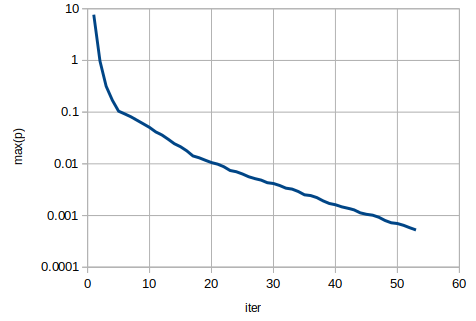
\includegraphics[width=0.6\linewidth]{linear2_simple_pres.png}
\end{center}


\subsubsection{Течение Пуазейля}
TODO

\subsubsection{Стационарное обтекание квадратного препятствия}

В тесте \ename{obstacle2-simple} из файла \ename{obstacle_simple_test.cpp}
рассматривается задача о стационарном обтекании
квадтратного препятствия (см. постановку в п. \ref{sec:problem-obstacle}).
По окончании расчёта в консоль печатаются коэффициенты сопротивления и подъёмной силы.

Используется естественная нумерация узлов с неактивными ячейками.
Класс \cvar{RegularGrid2D} предлагает следующие методы, связанные с неактивными ячейками:
\begin{itemize}
\item
\cvar{void RegularGrid2D::deactivate_cells(Point bot_left, Point top_right)} -- установить область неактивных ячеек;
\item
\cvar{bool RegularGrid2D::is_active_cell(size_t icell)} -- проверить, является ли ячейка активной.
\end{itemize}

Кроме того, в задаче появились внутренние границы.
То есть для постаноки граничных условий уже не достаточно
использовать крайние значение индексов $i$, $j$,
а нужен механизм для получения граничных отрезков сетки.
Для этого введены следующие функции
\begin{itemize}
\item
\cvar{RegularGrid2d::boundary_yfaces()} -- получить список всех вертикальных граничных фасок (возвращает парные индексы в
соответствии \cvar{yface_centered_grid}.
\item
\cvar{RegularGrid2d::boundary_xfaces()}  -- получить список всех горизонтальных граничных фасок (возвращает парные индексы в
соответствии \cvar{xface_centered_grid}.
\item
\cvar{RegularGrid2d::yface_type(size_t yface_index)} -- узнать тип вертикальной грани по её глобальному индексу.
Возвращает перечисление
\begin{minted}[linenos=false]{c++}
enum struct FaceType{
	Internal,     // внутренняя
	Boundary,     // граничная
	Deactivated   // неактивная (находится внутри неактивной области)
};
\end{minted}
\item
\cvar{RegularGrid2d::xface_type(size_t xface_index)} -- узнать тип вертикальной грани по её глобальному индексу.
\end{itemize}

\subsubsubsection{Функция верхнего уровня}
\clisting{open}{"test/obstacle_simple_test.cpp"}
\clisting{pass}{"TEST_CASE"}
Здесь сначала происходит установка параметров расчёта: числа Рейнольдса, параметра $E$,
количества итераций, порога сходимости и разбиения единичного интервала.
\clisting{lines-range}{"double Re", "n_unit"}
Далее строится сетка
\clisting{line}{"grid"}
В этом примере сетка строится в четырёхугольнике $[0, 12]\times[-2,2]$.
Потом для описания квадтратного препятствия 
происходит деактивация ячеек, находящихся в единичном квадрате
с нижней левой координатой $(2, -0.5)$ и верхней правой координатой $(3, 0.5)$.
\clisting{line}{"deactivate_cells"}
Потом создаётся решатель, инициализируются функции сохранения
и вызывается алгоритм потенциальной инициализации расчётных полей.
\clisting{until}{"worker.initialize();"}

Затем идёт стандартный цикл по SIMPLE-итерациям 
\clisting{block}{"size_t it = 0;"}

По окочании цикла вызывается функция сохранения решения в vtk
\clisting{line}{"worker.save_current_fields(it);"}

В конце происходит расчёт коэффициентов сил и их печать в консоль
\clisting{lines-range}{"coefs", "Cx"}
Результирующее поле течения сохраняется в файл \ename{obstacle2.vtk.series}.

\subsubsubsection{Учёт неактивных ячеек}
\clisting{to-start}{}
Неактивные ячейки учитываются во всех алгоритмах
сборки систем линейных уравнений. Рассмотрим на примере сборки
матрицы для пробной скорости, реализованной в функции \cvar{assemble_u_slae}.
\clisting{line}{"void Obstacle2DSimpleWorker::assemble_u_slae()"}
\clisting{pass}{"// internal"}
Рассмотрим цикл сборки внутренних узлов ``красной'' сетки для $u$
(или, что тоже самое, цикл по всем вертикальным граням основной сетки)
\clisting{lines-range}{"size_t j", "size_t i"}
Сначала вычисляется индекс строки (сквозной индекс текущей грани):
\clisting{line}{"row_index"}
Эта грань может быть либо внутренней, либо граничной (принадлежать внутренней вертикальной границе),
либо неактивной.
Выполняется проверка, является ли эта грань внутренней
\clisting{line}{"FaceType::Internal"}
Если да, то выполняется обычная процедура сборки
\clisting{before}{"else"}
Если нет (то есть грань либо неактивная, либо принадлежит внутренней границе),
то в диагональ ставится единица, в правую часть 0.
\clisting{block}{"else"}
Это отражает тот факт, что на внутренних границах $u=0$ из-за условий прилипания,
а для неактивных мы пишем тривиальное уравнение, просто чтобы матрица не была вырождена.

\clisting{to-start}{}
\clisting{pass}{"void Obstacle2DSimpleWorker::assemble_u_slae()"}
Учёт условий прилипания на внутренних горизонтальных
границах осуществляется через фиктивный узел в лямбда-функции \cvar{"add_to_mat"},
которая перехватывает все ситуации, когда алгоритм требует добавить что-либо в фиктивную колонку матрицы.
\clisting{line}{"auto add_to_mat"}
Такие ситуации могут произойти либо при сборке
около вертикальной грани, находящейся рядом с верхней границей:
\clisting{lines-range}{"if (ij_col[1] == _grid.ny())", "add_value"}
либо около вертикальной грани, находящейся рядом с нижней границей границей:
\clisting{lines-range}{"if (ij_col[1] == (size_t)-1)", "add_value"}
либо около вертикальнй грани, находящейся непосредственно над или под препятствием.
В этом случае индекс фиктивной колонки, в которую трубуется поставить будет
соответствовать неакотвной вертикальной грани.
Мы вычисляем этот индекс
\clisting{before}{"if"}
Если он неактивный, то следуем по процедуре добавления фиктивного узла около
границы с нулевым значением.
\clisting{block}{"if"}
Иначе -- это нормальная колонка и мы добавляем туда значение по стандартной процедуре
\clisting{line}{"add_value"}

\subsubsubsection{Расчёт коэффициентов сопротивления}
\label{sec:prog-cxcy}
\clisting{to-start}{}
Расчёт коэффициентов сил по формулам \cref{eq:ns2d_cx} осуществляется в процедуре \cvar{coefficients()}.
Она возвращает структуру, куда входят все шесть искомых значений
\clisting{block}{"struct Coefficients"}
Процедура, объявленная как
\clisting{line}{"Obstacle2DSimpleWorker::coefficients()"}
производит вычисления четырёх интегралов по простой квадратуре
\cref{eq:ns2d_gamma_quadrature}.
Результаты аггрегируются в переменные
\clisting{lines-range}{"sum_cpx", "sum_cfx"}
Операции проводятся в циклах по внутренним граничным отрезкам.
Сначала рассматриваются вертикальные границы:
\clisting{line}{"for (const RegularGrid2D::split_index_t& yface: _grid.boundary_yfaces())"}
Здесь в переменную \cvar{yface} попадают все парные индексы вертикальных граней, лежащих
на границах. Сначала нужно отфильтровать границы, лежащие во входном и выходном сечениях
\clisting{until}{" else "}
На вертикальных границах актуально вычисление коэффициентов $C^p_x$ (из пункта \ref{sec:compute-obstacle-coefs}).
Дли их определения на каждой сеточной грани мы должны определить
$p\,n_x$ по формулах \cref{eq:ns2d_obstacle_pnx_vertical}.
\clisting{line}{"pnx"}
Для использования этих формул нужно определить, является ли это левой или правой границей обтекаемого тела.
Мы вычисляем индексы ячеек, лежащих слева и справа.
Если левая ячейка активна, значит это левая граница, если правая активна, значит это правая граница.
\clisting{until}{"right_cell"}
Далее левой границы
\clisting{lines-range}{"if", "pnx"}
для правой
\clisting{lines-range}{"if", "pnx"}
иначе (если это и не правая и не левая граница) бросается исключение,
потому что так быть не должно: у любой внутренней границы должна быть хоть одна соседняя активная ячейка
\clisting{block}{"else"}
После вычисления $p\,n_x$ они добавляются
в искомые интегралы согласно
\cref{eq:ns2d_gamma_quadrature}:
\clisting{line}{"sum_cpx"}

Далее аналогичная процедура проводится для горизонтальных граней,
где актуально вычисление коэффициентов $C^f_x$.
Дли их определения на каждой сеточной грани мы должны определить
$\dsfr{u}{n}$ по формулах \cref{eq:ns2d_dudn_upper,eq:ns2d_dudn_lower}.

\clisting{block}{"for (const RegularGrid2D::split_index_t& xface: _grid.boundary_xfaces())"}

В конце функции искомые коэффициенты вычисляются через
уже найденные интегралы согласно
\cref{eq:ns2d_cx}:
\clisting{lines-range}{"Coefficients", "return"}

\subsubsubsection{Результаты расчёта}
Картина течения, полученная для
сетки \cvar{n_part = 10} при $\Ren = 20$,
представлена на \figref{fig:obstacle2-flow}
\begin{figure}[h!]
\centering
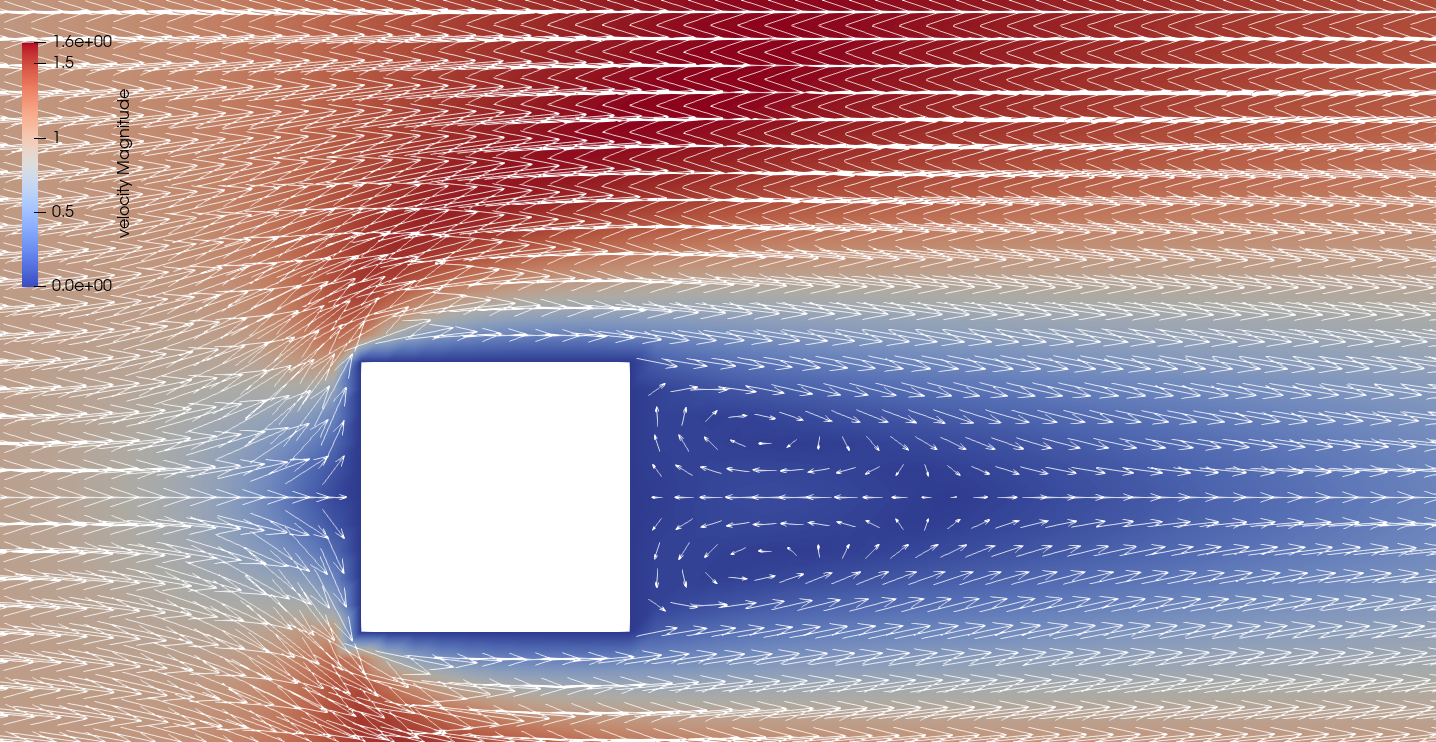
\includegraphics[width=0.9\linewidth]{obstacle2-flow.png}
\caption{Обтекание квадратного препятствия в стационарном режиме}
\label{fig:obstacle2-flow}
\end{figure}
Полученные коэффициенты сопротивления:
\begin{shelloutput}
=== Drag
Cpx = 2.97224
Cfx = 1.08639
Cx  = 4.05863
\end{shelloutput}
Для $\eps = 10^{-1}$ решение сошлось за 29 итераций.

\subsubsection{Нестационарное обтекание квадратного препятствия}
\label{sec:prob-obstacle-temp}

Эта задача реализована в файле \ename{obstacle_nonstat_simple_test.cpp}
в тесте \ename{[obstacle2-nonstat-simple]}.

Программа решает задачу в той же области, которая рассматривалась
в предыдущем пункте, но в нестационарной постановке
\cref{eq:ns2d_nonstat}

Поля течения для разных моментов времени пишутся в файл
\ename{obstacle-nonstat.vtk.series}. Кроме того, в файл \ename{c.txt}
пишутся вычисленные на разные моменты времени коэффициенты сопротивления.

\subsubsubsection{Функция верхнего уровня}
\clisting{open}{"test/obstacle_nonstat_simple_test.cpp"}
В начале обозначим параметры задачи:
числа Рейнольдса,
разбиение единичного отрезка,
шаг по времени $\dt$ и конечное время, 
параметр внутреннего итерационного процесса $E$, 
максимальное количество итераций во внутреннем итерационном процессе
и порог по невязке:
\clisting{pass}{"TEST_CASE"}
\clisting{lines-range}{"Re", "eps"}

Далее проводится создание сетки (так же, как и в предыдущем примере) и начальная инициализация
решателя
\clisting{lines-range}{"grid", "save_current_fields"}

После всех инициализаций начинается цикл по времени
\clisting{line}{"for (double time=time_step; time<end_time+1e-6; time+=time_step)"}
Отметим, что поскольку значению $t=0$ соответствует начальное
состояние решения, то цикл начинается сразу с первого шага $t=\dt$.

Внутри цикла по времени производится цикл
внутренних итераций SIMPLE
\clisting{block}{"size_t it"}

Далее, если текущее время кратно $1.0$, производится сохранение
решения в файл vtk и запись коэффициентов сил в файл:
\clisting{block}{"if"}

Печатается информация о сходимости текущей итерации
\clisting{line}{"cout"}

и производится переход на следующий шаг по времени:
\clisting{line}{"to_next_time_step"}

\subsubsubsection{Учёт нестационарности}
Согласно пунку \ref{sec:ns2d-nonstat} наличие производной по времени
учитывается:
\begin{itemize}
\item
При вычислении коэффициентов $d^u$, $d^v$
\cref{eq:ns2d_nonstat_duv}:
\clisting{to-start}{}
\clisting{pass}{"ObstacleNonstat2DSimpleWorker::ObstacleNonstat2DSimpleWorker("}
\clisting{lines-range}{"_du", "_dv"}
\item
При сборке систем уравнений для $u^*$, $u^*$
\cref{eq:ns2d_nonstat_uvstar}
\clisting{to-start}{}
\clisting{pass}{"void ObstacleNonstat2DSimpleWorker::assemble_u_slae()"}
как прибавка к диагонали
\clisting{line}{"add_to_mat(row_index, {i, j}, 1.0 + _tau/_time_step)"}
и правой части
\clisting{line}{"_rhs_u[row_index] += (_tau/_time_step)*_u_old[row_index]"}
\item
А так же в граничных условиях на выходе.
В этом случае условия \cref{eq:ns2d_outflow_common}
для $u$ по аналогии с \cref{eq:ns2d_outflow_common_semi}
аппроксимируются к виду
\begin{equation*}
(x,y)\in\Gamma_{out}:\; \frac{\hat u - \check u}{\dt} + \frac{\hat u - u}{\tau} + u\dfr{\hat u}{x} = 0.
\end{equation*}
Для упрощения по прежнему будем использовать ``стационарное'' условие
для поперечной скорости $v=0$.
Тогда для $u^*$ можно записать
$$
(x,y)\in\Gamma_{out}:\;
	\left(1 + \frac{\tau}{\dt}\right)u^*_{n_x, j+\tfrac12}
	+ \tau U_{n_x, j+\tfrac12}\frac{u^*_{n_x, j+\tfrac12}
					- u^*_{n_x-1, j+\tfrac12}}{h_x}
	= u_{n_x, j+\tfrac12}
	+ \frac\tau\dt \check u_{n_x, j+\tfrac12}
$$
Это выражение и добавляется в соответствующие строки матрицы и правой части
\clisting{to-start}{}
\clisting{pass}{"void ObstacleNonstat2DSimpleWorker::assemble_u_slae()"}
\clisting{block}{"// right boundary: du/dt + u*du/dx = 0"}
\item
При переходе на слудующий шаг по времени в функции
\clisting{to-start}{}
происходит вычисление текущего значения температуры, и
присваивание значений $\check u$, $\check v$.
\clisting{block}{"double ObstacleNonstat2DSimpleWorker::to_next_time_step()"}
Вызов \cvar{set_uvp} здесь осуществляется для пересборки актуальных матриц.

\end{itemize}

\subsection{Задание для самостоятельной работы}
\subsubsection{Расчитать коэффициент подъёмной силы}
Добавить расчёт коэффициентов подъёмной силы $C_y$ в
код для моделирования нестационарного обтекания (\ref{sec:prob-obstacle-temp}).
В п.(\ref{sec:prog-cxcy}) представлен используемый алгоритм
расчёта коэффицента сопротивления.
Отталкиваясь от этого алгоритма необходимо
\begin{itemize}
\item в класс \cvar{Coefficients} добавить поля \cvar{Cpy,Cfy,Cy},
\item добавить расчёт \cvar{dvdn} на вертикальных стенках препятствия по формулам  \cref{eq:ns2d_obstacle_dvdn_vertical},
\item добавить расчёт \cvar{pny} на горизонтальных стенках препятствия по формулам \cref{eq:ns2d_obstacle_pny_top,eq:ns2d_obstacle_pny_bot},
\item аггрегировать эти значения в \cvar{sum_cpy,sum_cfy}, из которых вычислить коэффициенты подъёмной силы,
\item сами коэффициенты добавить в файл \ename{c.txt}.
\end{itemize}


\subsubsection{Расчёт течения}
Провести расчёт течения при параметрах $\Ren = 100$, $\eps=10^{-1}$, $\dt = 0.1$, $t_{end} = 200$, $n=10$.
(для ускорения расчётов не забыть переключиться на релизную сборку).
\begin{itemize}
\item Показать динамику изменения расчётных полей: скалярных $p$, $|\vec v|$ и вектора скорости $\vec v$,
\item Нарисовать графики изменения коэффициентов сопротивления $C_x, C^p_x, C^f_x$ и подъёмной силы $C_y, C^p_y, C^f_y$ во времени.
\end{itemize}
